\documentclass[preprint,12pt]{elsarticle}
%% Elsevier template. Suitable targets include Computer Methods and Programs in
%% Biomedicine Update, SoftwareX (shortened), International Journal of Medical
%% Informatics, or (BMC template) Journal of Biomedical Semantics / BMC Medical
%% Informatics and Decision Making.

\usepackage[T1]{fontenc}
\usepackage[utf8]{inputenc}
\usepackage{lmodern}
\usepackage{amsmath,amssymb}
\usepackage{graphicx}
\usepackage{booktabs}
\usepackage{array}
\usepackage{xcolor}
\usepackage{tikz}
\usetikzlibrary{positioning,arrows.meta,fit,calc}
\usepackage[hidelinks]{hyperref}
\usepackage{url}
\setlength{\emergencystretch}{2em}

\journal{Comput. Methods Programs Biomed. Update}

\begin{document}

\begin{frontmatter}

\title{EpiFHIR: an open, reproducible pipeline that links epilepsy records to an ontology and HL7 FHIR R4, evaluated end to end on public synthetic patients}

\author[vit]{M.\,J. Yogesh\corref{cor1}}
\ead{yogeshmj.nie@gmail.com}
\author[vit]{Karthikeyan J.\corref{cor1}}
\ead{karthikeyan.jk@vit.ac.in}
\cortext[cor1]{Corresponding authors.}
\affiliation[vit]{organization={School of Computer Science Engineering and Information Systems, Vellore Institute of Technology},
            city={Vellore}, postcode={632 014}, state={Tamil Nadu}, country={India}}

\begin{abstract}
\noindent\textbf{Background and objective:} Epilepsy data rarely travel well. Seizure types are written in free text, coded too coarsely, and locked into local schemas. Many published pipelines that claim to fix this cannot be rerun, because the patient data behind them cannot be shared. We built EpiFHIR, an open pipeline that maps epilepsy terms to an ontology, exports the result as HL7 FHIR R4, and stores it for analysis, and we evaluated it using only public inputs so that anyone can reproduce every number.

\noindent\textbf{Methods:} Terms are aligned to the Epilepsy Ontology (EPIO; 1,915 classes, 250 derived from EpSO) in three stages: normalisation and lemmatisation, prefix-trie candidate retrieval, and character n-gram scoring with an abstention threshold. We tested alignment on 423 held-out ontology synonyms, on perturbed versions of them, and on the 95 entries of the ICD-10-CM G40 hierarchy. We generated 2,095 synthetic patients with a seizure disorder using Synthea, exported them to FHIR R4, validated every bundle with the HAPI FHIR validator, and compared the output with Synthea's independent FHIR exporter. We also benchmarked SQLite against PostgreSQL and ran negative and positive controls for the prediction layer.

\noindent\textbf{Results:} At a threshold chosen on a separate tuning set, alignment reached 70.1\% precision and 49.9\% recall (F1 0.583), against F1 0.446 for word TF-IDF retrieval, 0.390 for fuzzy matching and 0.042 for exact matching. All 2,095 bundles (22,606 resources) passed HAPI validation without errors, and records agreed exactly with Synthea's own exporter for every patient. With an outcome unrelated to patient features, models scored AUROC 0.514 and 0.499; with an injected effect of known size (oracle AUROC 0.802), they recovered 0.803 and 0.794.

\noindent\textbf{Conclusions:} The interoperability layer is reliable. Ontology alignment by lexical means is useful but recovers only about half of unseen synonyms, and text-only mappings can be confidently wrong, so they need review before clinical use. All code, data-generation settings and results are released for reuse and for validation on real records.
\end{abstract}

\begin{highlights}
\item An open pipeline links epilepsy terms to an ontology and exports HL7 FHIR R4.
\item All 2,095 synthetic patient bundles passed HAPI FHIR R4 validation with no errors.
\item Exports matched an independent FHIR implementation for every patient.
\item Lexical alignment recovered 50\% of unseen ontology synonyms at 70\% precision.
\item Negative and positive controls show the analytics layer adds no spurious signal.
\end{highlights}

\begin{keyword}
Epilepsy \sep HL7 FHIR \sep Ontology alignment \sep Synthetic data \sep Reproducibility \sep Interoperability
\end{keyword}

\end{frontmatter}

%% ===========================================================================
\section{Introduction}
\label{sec:intro}

Consider a patient who has a convulsion at home and is brought to an emergency department. The note says ``GTC, post-ictal, known epilepsy on clonazepam''. Their neurologist writes ``generalised tonic-clonic seizure'' three weeks later, and the discharge code is a broad ICD-10 epilepsy code. Each record is correct, and none of them can easily be matched to the others. Multiply this by every hospital, and it becomes clear why epilepsy, a condition that affects more than 50 million people \cite{who2019}, is still hard to monitor at population scale.

The tools to fix this exist. The International League Against Epilepsy (ILAE) publishes a seizure classification \cite{fisher2017}. Epilepsy ontologies such as EpSO \cite{sahoo2014} and the community-built Epilepsy Ontology (EPIO) \cite{sargsyan2023} define the concepts and their synonyms. HL7 FHIR R4 \cite{fhir} gives a shared format for exchanging the resulting data. What is missing is a pipeline that joins these pieces and that other groups can actually check.

That last point matters more than it may seem. Epilepsy informatics papers often report strong results on hospital records that readers cannot access, and the code needed to reproduce them is often missing or incomplete. A reviewer then has no way to tell a working system from one that only looks good on paper. We therefore took a deliberately conservative approach. We built the pipeline first and evaluated every component on inputs that anyone can download: a public ontology, the public ICD-10-CM code set \cite{icd10cm}, and synthetic patients from Synthea \cite{walonoski2018}. Synthetic data cannot tell us whether a clinical prediction is accurate, and we make no such claim. They can tell us, precisely and repeatably, whether the software does what it says.

This paper describes EpiFHIR and reports five experiments, each tied to one question:
\begin{itemize}
\item \textbf{RQ1, alignment.} How well does three-stage lexical alignment map unseen epilepsy terms to the right ontology class, compared with standard string-matching baselines?
\item \textbf{RQ2, robustness.} How much does accuracy drop when terms contain typos, reordered words or different inflections?
\item \textbf{RQ3, conformance.} Do the exported FHIR R4 bundles pass an independent validator, and does that validator actually catch errors?
\item \textbf{RQ4, fidelity.} Does the export agree with an independent FHIR implementation working from the same records?
\item \textbf{RQ5, analytics.} Do the storage and prediction layers behave correctly, and do they avoid inventing signal?
\end{itemize}

We also report what went wrong along the way. Several of the most useful findings, including a confidently wrong mapping that propagated to thousands of records, came from failures rather than successes.

%% ===========================================================================
\section{Background}
\label{sec:background}

\paragraph{Epilepsy ontologies} EpSO organises epilepsy knowledge along four dimensions (seizure type, anatomical location, etiology and associated conditions) and follows ILAE terminology \cite{sahoo2014}. It underpinned EpiDEA, which extracted structured epilepsy information from discharge summaries \cite{cui2012}, and later work used it to engineer features for classifying neuropathology reports \cite{sahoo2022}. EPIO is a larger, community-maintained ontology built to BFO and OBO principles; it incorporates EpSO-derived classes and adds synonyms and cross-references to SNOMED CT, ICD-10-CM, UMLS and MeSH \cite{sargsyan2023}. We use EPIO because it can be downloaded openly under the MIT licence, which keeps the whole evaluation reproducible.

\paragraph{Concept alignment} General tools such as MetaMap \cite{aronson2001}, QuickUMLS \cite{soldaini2016} and scispaCy \cite{neumann2019} map text to the UMLS. They require UMLS licences or large model downloads, and they target the UMLS rather than an epilepsy ontology, so we compare against simpler baselines that need neither. Transformer language models have since improved clinical extraction, for example of seizure frequency from clinic notes \cite{xie2022}, at the cost of annotated training data and heavier infrastructure.

\paragraph{Interoperability} FHIR represents clinical data as typed resources exchanged through a REST API \cite{fhir,braunstein2018}. SMART on FHIR lets applications run inside commercial EHRs \cite{mandel2016}, and research repositories such as i2b2 can serve their data as FHIR \cite{wagholikar2017}. The ILAE Big Data Task Force has called for exactly this combination of shared vocabularies and standard formats in epilepsy \cite{lhatoo2020}. Billing codes alone are a weak substitute: they identify epilepsy reasonably well \cite{jette2010} but say little about seizure type or treatment.

%% ===========================================================================
\section{System design}
\label{sec:design}

EpiFHIR has four layers (Fig.~\ref{fig:arch}). It is written in Python, uses no proprietary components, and runs on a laptop.

\begin{figure}[t]
\centering
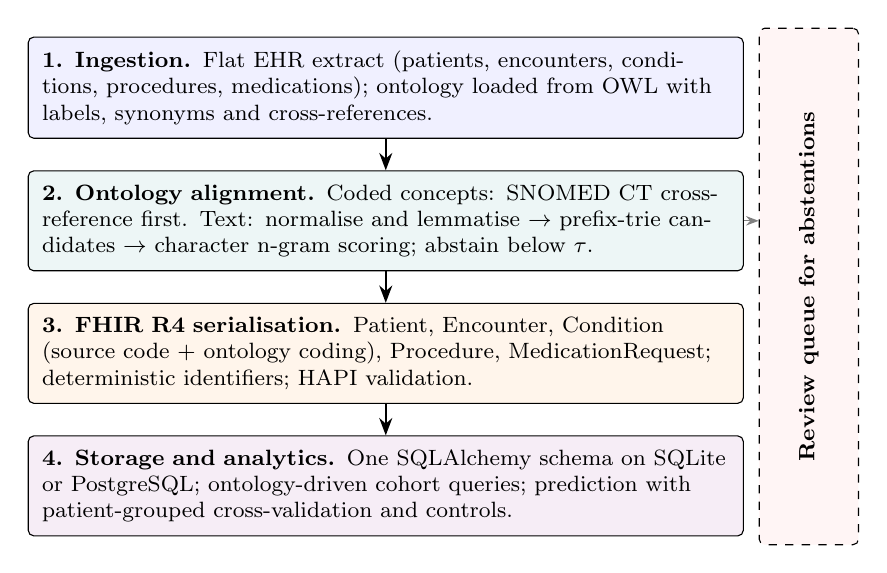
\begin{tikzpicture}[
  box/.style={draw, rounded corners=2pt, fill=#1, text width=0.72\linewidth, align=left, inner sep=5pt, font=\footnotesize},
  box/.default=gray!8, arr/.style={-{Stealth[length=2.2mm]}, thick}, node distance=4mm]
\node[box=blue!6] (A) {\textbf{1. Ingestion.} Flat EHR extract (patients, encounters, conditions, procedures, medications); ontology loaded from OWL with labels, synonyms and cross-references.};
\node[box=teal!7, below=of A] (B) {\textbf{2. Ontology alignment.} Coded concepts: SNOMED CT cross-reference first. Text: normalise and lemmatise $\rightarrow$ prefix-trie candidates $\rightarrow$ character n-gram scoring; abstain below $\tau$.};
\node[box=orange!8, below=of B] (C) {\textbf{3. FHIR R4 serialisation.} Patient, Encounter, Condition (source code + ontology coding), Procedure, MedicationRequest; deterministic identifiers; HAPI validation.};
\node[box=violet!7, below=of C] (D) {\textbf{4. Storage and analytics.} One SQLAlchemy schema on SQLite or PostgreSQL; ontology-driven cohort queries; prediction with patient-grouped cross-validation and controls.};
\foreach \a/\b in {A/B,B/C,C/D} \draw[arr] (\a) -- (\b);
\node[draw, dashed, rounded corners=2pt, fill=red!4, inner sep=3pt,
      fit={($(A.north east)+(0.3,0)$) ($(D.south east)+(1.35,0)$)}] (V) {};
\node[rotate=90, font=\footnotesize\bfseries, align=center] at (V.center) {Review queue for abstentions};
\draw[-{Stealth[length=1.6mm]}, gray] (B.east) -- (V.west |- B.east);
\end{tikzpicture}
\caption{EpiFHIR architecture. Terms the aligner cannot match confidently go to a review queue instead of being forced onto a class.}
\label{fig:arch}
\end{figure}

\subsection{Ontology loading}
The loader reads an OWL file with rdflib and keeps, for each class, its label, its exact and related synonyms, and its database cross-references, normalised by coding system. EPIO (commit \texttt{dc9f9b1}, January 2023) yields 1,915 classes with 2,323 exact synonyms that differ from their labels. Of these classes, 250 are marked as derived from EpSO. Cross-references cover SNOMED CT for 321 classes, ICD-10-CM for 148, ICD-9-CM for 108, UMLS for 634 and MeSH for 362.

\subsection{Three-stage alignment}
\textit{Stage 1, normalisation.} Text is folded to ASCII, lower-cased, split into alphanumeric tokens, stripped of a short stop-word list (articles, prepositions and words such as ``disorder'' or ``unspecified'' that carry little meaning in this domain), and lemmatised with simplemma, so that ``seizures'' and ``seizure'' coincide. If the normalised form matches exactly one indexed form, the aligner returns that class.

\textit{Stage 2, candidate retrieval.} Every normalised token of every surface form is indexed in an inverted index, and the vocabulary is stored in a prefix trie. A query token that is not in the vocabulary is completed through the trie (prefixes of at least four characters), which lets partial and misspelled words still retrieve candidates. The candidate set is the union of forms sharing at least one token with the query.

\textit{Stage 3, scoring.} Candidates are ranked by the cosine similarity between character 3--5-gram TF-IDF vectors of the query and of each surface form,
\begin{equation}
s(q,f)=\frac{\mathbf{v}_q\cdot\mathbf{v}_f}{\lVert\mathbf{v}_q\rVert_2\,\lVert\mathbf{v}_f\rVert_2},
\end{equation}
and the class of the best form is returned if $s\ge\tau$. Otherwise the aligner abstains and the term goes to manual review. Character n-grams tolerate spelling variation and need no external embeddings, which keeps the method small and fully reproducible.

\subsection{FHIR R4 serialisation}
The exporter builds one FHIR \texttt{collection} bundle per patient. Condition resources keep the source SNOMED CT coding and add an ontology coding: through the ontology's own SNOMED cross-reference when one exists, and otherwise through text alignment of the condition name. Identifiers are deterministic (UUID version 5) and the ontology is processed in sorted order, so re-running the export gives byte-identical output.

\subsection{Storage}
A single SQLAlchemy schema (patients, encounters, conditions with an ontology column, medications) runs unchanged on SQLite, for single-user analysis, and on PostgreSQL, for multi-user deployments.

%% ===========================================================================
\section{Evaluation design}
\label{sec:eval}

All experiments ran on a two-core virtual machine (Intel Xeon, 2.1\,GHz, 7\,GB RAM) with Python 3.13, Java 21, SQLite 3.53 and PostgreSQL 16. Random seeds are fixed throughout.

\subsection{Data}
\paragraph{Synthetic patients} We ran Synthea \cite{walonoski2018} (build \texttt{bd8a52b}) with its epilepsy module and a filter that keeps only patients who develop a seizure disorder (SNOMED CT 128613002), using seed 42 and the Massachusetts demographic model. This produced 2,095 patients. In this module, patients develop a seizure disorder, have emergency visits for seizures, undergo EEG, receive one of three antiseizure medications (carbamazepine, diazepam or clonazepam), and in some cases are diagnosed with epilepsy (SNOMED CT 84757009). Synthea wrote each patient both as flat CSV files, our pipeline's input, and as FHIR R4 bundles produced by its own exporter, which we used as an independent reference.

\paragraph{Benchmark A: held-out synonyms} For each of the 876 EPIO classes with at least one exact synonym, we drew one synonym at random, removed it from the index, and used it as a query whose correct answer is its class. Because EPIO imports anatomy, phenotype and disease classes from other ontologies, these queries include neighbouring clinical terms as well as epilepsy-specific ones. We excluded 30 queries whose normalised text was identical to a form of a different class, because their correct answer is undefined. The remaining 846 queries were split at random into a tuning set (423), used only to choose thresholds, and a test set (423), used once for reporting. In 39 test queries, normalisation reduces the held-out synonym to a form still indexed for its class; we report results with and without them.

\paragraph{Benchmark A$'$: perturbations} Each test query was also modified in four ways: changed case and punctuation, reversed word order, changed inflection of the final word, and a single transposition of adjacent letters in the longest word.

\paragraph{Benchmark B: ICD-10-CM titles} We aligned the titles of all 95 entries in the ICD-10-CM G40 hierarchy (the G40--G47 block heading and 94 G40 codes). ICD-10-CM, the US clinical modification, has no G41 category; status epilepticus is coded within G40. We first intended to use EPIO's ICD-10-CM cross-references as gold labels but found that they encode ``classified under'' rather than equivalence; Landau--Kleffner syndrome, for example, is cross-referenced to G40.8 (``other epilepsy''). We therefore report how many titles were aligned and, where possible, whether the predicted class cross-references the code or one of its ancestors.

\subsection{Baselines}
\textit{Exact match} compares lower-cased strings. \textit{Fuzzy matching} returns the nearest surface form by rapidfuzz WRatio. \textit{Word TF-IDF retrieval} ranks forms by cosine similarity of word unigram and bigram vectors. Each baseline's acceptance threshold, and EpiAlign's $\tau$ (searched from 0.30 to 0.90 in steps of 0.05), was chosen to maximise F1 on the tuning set.

\subsection{Metrics}
For alignment, \textit{coverage} is the share of queries for which a class was returned, \textit{precision} the share of returned classes that were correct, and \textit{recall} the share of all queries answered correctly. Proportions carry Wilson 95\% confidence intervals. FHIR conformance was checked with the HAPI FHIR instance validator \cite{hapi} (version 6.1.0) against the base R4 StructureDefinitions, offline and with terminology checks disabled. To confirm that the validator detects errors at all, we also validated deliberately corrupted copies of one bundle. Fidelity was measured as the Jaccard overlap between the (code, date) pairs in our bundles and in Synthea's bundles for the same patient.

\subsection{Prediction controls}
The prediction layer is evaluated with controls rather than headline accuracy, because in Synthea's epilepsy module the chance of a further seizure visit is fixed at 20\% per treatment cycle and does not depend on any patient attribute. The unit of analysis was a seizure-related emergency encounter, and the outcome was another such encounter within 365 days. Encounters whose follow-up ended earlier without an event were excluded. Thirteen features described demographics, prior seizure visits, time since the last visit, diagnoses and current medication. Logistic regression and XGBoost \cite{chen2016} were evaluated with five-fold cross-validation grouped by patient (scikit-learn \cite{pedregosa2011}), AUROC confidence intervals from 1,000 patient-level bootstrap samples, and label permutation (50 permutations for logistic regression, 10 for XGBoost). In the \textit{negative control} the true outcome was used and the expected AUROC is 0.5. In the \textit{positive control} we replaced the outcome with one drawn from a logistic model in which prior seizure visits and age had known effects (1.2 and 0.6 log-odds per standard deviation), so that the best achievable AUROC could be computed exactly.

%% ===========================================================================
\section{Results}
\label{sec:results}

\subsection{RQ1: alignment of unseen synonyms}
Table~\ref{tab:align} and Fig.~\ref{fig:align}a summarise the test set. The tuning set selected $\tau=0.65$. At that threshold EpiAlign answered 71.2\% of queries, was right 70.1\% of the time when it answered, and recovered 49.9\% of all queries correctly (F1 0.583). Word TF-IDF retrieval and fuzzy matching answered more queries but were wrong more often, with F1 of 0.446 and 0.390. Exact matching was never wrong but answered only 9 of 423 queries. Excluding the 39 queries that normalisation makes trivial, EpiAlign's precision was 66.0\% and recall 45.1\% (F1 0.536).

\begin{table}[t]
\centering
\caption{Alignment of 423 held-out EPIO synonyms (test set). Thresholds were chosen on a separate tuning set. Precision and recall in \% with Wilson 95\% CI.}
\label{tab:align}
\footnotesize
\setlength{\tabcolsep}{4pt}
\resizebox{\linewidth}{!}{%
\begin{tabular}{@{}lcccccc@{}}
\toprule
Method & Threshold & Coverage & Precision & Recall & F1 & ms/query \\
\midrule
%% generated from results: tables/align_main.tex
\textbf{EpiAlign (this work)} & 0.65 & 71.2 & 70.1 (64.7--75.0) & 49.9 (45.1--54.6) & 0.583 & 0.61 \\
Word TF-IDF retrieval & 0.40 & 83.2 & 49.1 (44.0--54.4) & 40.9 (36.3--45.6) & 0.446 & 0.66 \\
Fuzzy matching (WRatio) & 0.75 & 91.7 & 40.7 (35.9--45.7) & 37.4 (32.9--42.1) & 0.390 & 4.09 \\
Exact string match & -- & 2.1 & 100.0 (70.1--100.0) & 2.1 (1.1--4.0) & 0.042 & 0.00 \\
\bottomrule
\end{tabular}}
\end{table}

The threshold works as a dial between automation and review (Fig.~\ref{fig:align}b). At $\tau=0.30$ the aligner answers 90.3\% of queries at 61.3\% precision; at $\tau=0.90$ it answers 25.8\% at 89.9\% precision. F1 changes little between 0.30 and 0.70 (0.569--0.589), so the choice of threshold is really a choice of how much manual review a site can afford.

\begin{figure}[t]
\centering
\includegraphics[width=\linewidth]{figures/fig_alignment.pdf}
\caption{(a) Precision, recall and F1 of each method on the test set. (b) EpiAlign precision, recall, coverage and F1 as the threshold $\tau$ varies; the dotted line marks the value chosen on the tuning set.}
\label{fig:align}
\end{figure}

Table~\ref{tab:ablation} removes one component at a time. Stage 3 is the main source of recall: replacing character n-gram scoring with token overlap raised precision to 79.6\% but cut recall almost in half, to 27.7\%. Lemmatisation added 1.9 points of recall. The trie did not change accuracy (F1 0.583 with it, 0.587 without); its job is speed, and scanning every form instead took 1.70\,ms per query rather than 0.61\,ms, a 2.8-fold slowdown that will grow with larger ontologies. Indexing EPIO's related synonyms as well as its exact ones made no meaningful difference.

\begin{table}[t]
\centering
\caption{Ablation of EpiAlign on the test set ($\tau=0.65$). Values in \%, except F1 and time.}
\label{tab:ablation}
\footnotesize
\begin{tabular}{@{}lccccc@{}}
\toprule
Configuration & Coverage & Precision & Recall & F1 & ms/query \\
\midrule
%% generated from results: tables/align_ablation.tex
Full pipeline & 71.2 & 70.1 & 49.9 & 0.583 & 0.61 \\ \midrule
Without lemmatisation & 68.6 & 70.0 & 48.0 & 0.569 & 0.60 \\
Without trie (scan all forms) & 72.3 & 69.9 & 50.6 & 0.587 & 1.70 \\
Without Stage 3 (token Jaccard) & 34.8 & 79.6 & 27.7 & 0.411 & 0.06 \\
Adding related synonyms to index & 74.0 & 68.4 & 50.6 & 0.582 & 0.56 \\
\bottomrule
\end{tabular}
\end{table}

\subsection{RQ2: robustness}
Normalisation made EpiAlign indifferent to case, punctuation and word order: recall stayed at 49.9\% under both perturbations, whereas fuzzy matching lost 10.0 and 3.6 points (Fig.~\ref{fig:robust}). Changing the final word's inflection cost EpiAlign 2.6 points. A single transposed letter was the hardest case for every method: EpiAlign fell to 28.1\%, and the two approximate baselines to 26.2--26.5\%. Typos break the exact-match shortcut and corrupt several character n-grams at once, which points to a spelling-correction step as a cheap improvement.

\begin{figure}[t]
\centering
\includegraphics[width=\linewidth]{figures/fig_robustness.pdf}
\caption{Recall on the 423 test queries before and after each perturbation.}
\label{fig:robust}
\end{figure}

\subsection{Alignment of ICD-10-CM titles}
On the 95 ICD-10-CM G40 titles, EpiAlign aligned 55 and abstained on 40 (Table~\ref{tab:icd}). Its failures were systematic and instructive. About half of the abstentions (21 of 40) were the long ``Localization-related (focal) (partial) \ldots\ epilepsy and epileptic syndromes with \ldots'' titles, whose wording matches no single ontology label. Of the aligned titles, 20 were mapped to EPIO's ``Intractable Epilepsy'' class, because the qualifier ``intractable'' outweighed the head concept. Few judgements could be checked: only 4 of EpiAlign's 55 predictions point to a class that carries any ICD-10-CM cross-reference. The sparseness of these cross-references, rather than any one algorithm, is the main obstacle to automated ICD-to-ontology mapping today.

\begin{table}[t]
\centering
\caption{Alignment of the 95 ICD-10-CM G40 titles. \textit{Consistent}: the predicted class cross-references the code or an ancestor; \textit{inconsistent}: it cross-references only other codes; \textit{unverifiable}: it has no ICD-10-CM cross-reference.}
\label{tab:icd}
\footnotesize
\begin{tabular}{@{}lccccc@{}}
\toprule
Method & Aligned & Abstained & Consistent & Inconsistent & Unverifiable \\
\midrule
%% generated from results: tables/icd.tex
EpiAlign & 55 & 40 & 1 & 3 & 51 \\
Word TF-IDF & 75 & 20 & 1 & 8 & 66 \\
Fuzzy (WRatio) & 95 & 0 & 6 & 50 & 39 \\
Exact match & 3 & 92 & 0 & 0 & 3 \\
\bottomrule
\end{tabular}
\end{table}

\subsection{RQ3: FHIR conformance}
The 2,095 synthetic patients had a median age of 6.0 years (IQR 0.7--12.9) at their first seizure-disorder diagnosis; 1,097 were female, 1,101 were also diagnosed with epilepsy, and 630 had died by the end of the simulation. They had 3,341 seizure-related emergency visits, each with an EEG, and 5,697 antiseizure-medication orders (clonazepam 1,954, diazepam 1,937, carbamazepine 1,806).

EpiFHIR exported them as 2,095 bundles containing 22,606 resources (Table~\ref{tab:fhir}) in a median of 3.8\,ms per patient (95th percentile 5.7\,ms). Every bundle passed HAPI validation against the base R4 specification with zero errors and zero warnings. A clean result means little unless the validator can fail, so we corrupted copies of one bundle (Table~\ref{tab:sanity}). HAPI caught a missing required element, an impossible date, an undefined element and a wrong datatype. It did not catch a status code outside the required value set, because terminology checks were disabled offline. Base-R4 validation is therefore necessary but not sufficient, and production deployments should add a terminology server.

For comparison, all 100 randomly sampled Synthea bundles produced validation errors (15,905 messages in total). Every one of these messages was the same kind: a reference to a US Core profile that cannot be resolved offline. None reported a structural problem.

\begin{table}[t]
\centering
\begin{minipage}[t]{0.38\linewidth}
\centering
\caption{Resources exported.}
\label{tab:fhir}
\footnotesize
\begin{tabular}{@{}lr@{}}
\toprule
Resource & Count \\
\midrule
%% generated from results: tables/resources.tex
Patient & 2,095 \\
Encounter & 6,182 \\
Condition & 5,291 \\
Procedure & 3,341 \\
MedicationRequest & 5,697 \\
\midrule Total & 22,606 \\
\bottomrule
\end{tabular}
\end{minipage}\hfill
\begin{minipage}[t]{0.58\linewidth}
\centering
\caption{Validator check on corrupted copies of one bundle.}
\label{tab:sanity}
\footnotesize
\begin{tabular}{@{}p{0.56\linewidth}cc@{}}
\toprule
Fault injected & Errors & Caught \\
\midrule
%% generated from results: tables/sanity.tex
None (exported bundle) & 0 & -- \\
Required element removed (MedicationRequest.status) & 1 & yes \\
Impossible date (2021-13-45) & 2 & yes \\
Undefined element added & 1 & yes \\
Wrong datatype (birthDate as number) & 3 & yes \\
Status value outside required value set & 0 & no \\
\bottomrule
\end{tabular}
\end{minipage}
\end{table}

\subsection{RQ4: fidelity against an independent implementation}
Synthea's FHIR exporter and EpiFHIR share no code; ours works from the CSV extract. For every one of the 2,095 patients, the two produced identical sets of conditions, medication requests and procedures (Table~\ref{tab:conc}). Reaching this result exposed a trap that would have looked like a data-loss bug: Synthea writes FHIR timestamps in the generating machine's local time zone (here UTC+05:30), condition dates in the CSV in that same zone, and other CSV timestamps in UTC. Comparing raw strings suggested that 22\% of medication orders disagreed. Comparing instants showed that none did.

\begin{table}[t]
\centering
\caption{Agreement between EpiFHIR and Synthea's own FHIR export. Medication and procedure times compared as UTC instants; condition onsets as calendar dates.}
\label{tab:conc}
\footnotesize
\resizebox{\linewidth}{!}{%
\begin{tabular}{@{}lccccc@{}}
\toprule
Resource & EpiFHIR & Synthea & Shared & Jaccard & Identical patients \\
\midrule
%% generated from results: tables/concordance.tex
Condition & 5,291 & 5,291 & 5,291 & 1.000 & 2,095/2,095 \\
MedicationRequest & 5,697 & 5,697 & 5,697 & 1.000 & 2,095/2,095 \\
Procedure & 3,341 & 3,341 & 3,341 & 1.000 & 2,095/2,095 \\
\bottomrule
\end{tabular}}
\end{table}

The ontology coding step attached an EPIO class to all 5,291 conditions, but only one of the three distinct condition codes was mapped through a cross-reference (Epilepsy $\rightarrow$ EPIO ``epilepsy''). The other two were mapped by text alignment. ``Seizure disorder'' became EPIO ``seizure'', which is close but describes an event rather than a disorder. ``History of seizure'' became the generic class ``history'', which is simply wrong. Because each code appears once per patient, these two text mappings were copied onto 4,190 condition records. Alignment errors behave very differently on coded data than in a benchmark: one wrong decision is repeated thousands of times. The released exporter therefore defaults to sending coded concepts that lack a cross-reference to the review queue instead of mapping them by text; the automatic behaviour evaluated here remains available as an option.

\subsection{RQ5: storage and prediction}
Table~\ref{tab:storage} and Fig.~\ref{fig:storage} compare the two back ends as the cohort was replicated to 10,475 and 41,900 patients (up to 1.69 million rows). On this single machine SQLite was faster on every measure: bulk loading at 91--136 thousand rows per second against 29--33 thousand for PostgreSQL, ontology cohort queries in 132\,ms against 195\,ms at the largest size, and 4,588--5,156 concurrent commits per second from four threads against 2,167--2,486. Neither back end produced write errors once a benchmark bug was fixed. That bug is itself worth reporting: our test wrote 45-character identifiers into a 40-character column. PostgreSQL rejected all 2,000 writes, and SQLite, which does not enforce declared lengths, silently accepted them. PostgreSQL's advantages lie in what this test does not measure: network access by many clients, access control and operational tooling.

\begin{table}[t]
\centering
\caption{Storage benchmark. Load in thousands of rows per second; cohort query is the median of five runs; record retrieval is the median / 95th percentile over 300 patients; concurrent writes are single-row commits per second from four threads (errors in parentheses).}
\label{tab:storage}
\footnotesize
\setlength{\tabcolsep}{3.5pt}
\resizebox{\linewidth}{!}{%
\begin{tabular}{@{}lrrrrcc@{}}
\toprule
Back end & Patients & Rows & Load & Query (ms) & Record (ms) & Commits/s \\
\midrule
%% generated from results: tables/storage.tex
SQLite & 2,095 & 84,470 & 135.9 & 6.2 & 0.29 / 0.58 & 4,588 (0) \\
PostgreSQL & 2,095 & 84,470 & 33.4 & 7.6 & 1.79 / 2.70 & 2,168 (0) \\
SQLite & 10,475 & 422,350 & 120.5 & 28.3 & 0.30 / 0.41 & 5,156 (0) \\
PostgreSQL & 10,475 & 422,350 & 33.2 & 36.9 & 0.77 / 1.82 & 2,486 (0) \\
SQLite & 41,900 & 1,689,400 & 91.1 & 131.6 & 0.30 / 0.54 & 5,110 (0) \\
PostgreSQL & 41,900 & 1,689,400 & 28.9 & 195.3 & 1.83 / 2.55 & 2,167 (0) \\
\bottomrule
\end{tabular}}
\end{table}

\begin{figure}[t]
\centering
\includegraphics[width=\linewidth]{figures/fig_storage.pdf}
\caption{(a) Bulk-load throughput, (b) ontology-driven cohort query latency and (c) concurrent commit throughput for SQLite and PostgreSQL.}
\label{fig:storage}
\end{figure}

The prediction data comprised 3,069 index encounters from 1,932 patients, 810 (26.4\%) followed by another seizure visit within a year. As designed, the negative control found nothing (Table~\ref{tab:pred}, Fig.~\ref{fig:pred}a). Logistic regression reached AUROC 0.514 (95\% CI 0.491--0.537) and XGBoost 0.499 (0.477--0.521), both within the range of label permutations (permutation $p=0.24$ and $0.73$), and neither improved the Brier score over predicting the base rate. In the positive control, where the best achievable AUROC was 0.802, logistic regression recovered 0.803 (0.785--0.821) and XGBoost 0.794 (0.772--0.813) (Fig.~\ref{fig:pred}b). Together the two controls show that the pipeline finds signal when it exists and does not manufacture it when it does not, which a single headline AUROC cannot show.

\begin{table}[t]
\centering
\caption{Prediction controls. AUROC with patient-level bootstrap 95\% CI; Brier score of the model and of a constant base-rate prediction; mean AUROC under label permutation.}
\label{tab:pred}
\footnotesize
\setlength{\tabcolsep}{4pt}
\resizebox{\linewidth}{!}{%
\begin{tabular}{@{}llcccc@{}}
\toprule
Control & Model & AUROC (95\% CI) & Brier & Base-rate Brier & Permuted AUROC \\
\midrule
%% generated from results: tables/prediction.tex
Negative & Logistic regression & 0.514 (0.491--0.537) & 0.195 & 0.194 & 0.498 \\
Negative & XGBoost & 0.499 (0.477--0.521) & 0.199 & 0.194 & 0.507 \\
Positive & Logistic regression & 0.803 (0.785--0.821) & 0.148 & 0.206 & 0.500 \\
Positive & XGBoost & 0.794 (0.772--0.813) & 0.151 & 0.206 & 0.495 \\
\bottomrule
\end{tabular}}
\end{table}

\begin{figure}[t]
\centering
\includegraphics[width=\linewidth]{figures/fig_prediction.pdf}
\caption{Out-of-fold ROC curves. (a) Negative control: the outcome does not depend on any feature. (b) Positive control: an outcome with known effects whose best achievable AUROC is 0.802.}
\label{fig:pred}
\end{figure}

%% ===========================================================================
\section{Discussion}
\label{sec:discussion}

EpiFHIR's interoperability layer did what it should. Every bundle was valid, every record matched an independent implementation, and the validator was shown to catch the faults it claims to catch. The ontology layer is more modest. Lexical alignment beat the standard string-matching baselines by a clear margin, but it still recovered only about half of unseen synonyms, and its errors on coded data were repeated at scale.

\subsection{Six lessons from building it}
\textit{1. Synonyms are harder than spelling.} Many held-out synonyms share almost no characters with the label they belong to. EpiAlign missed ``non-epileptic attack disorder'' (gold: psychogenic non-epileptic seizure) and ``vitamin B6-dependent seizures'' (gold: pyridoxine-dependent epilepsy), and every acronym we inspected, such as LTLE, MTLE-HS and IHHS, scored zero. No lexical method can bridge that gap, which is why no method in Table~\ref{tab:align} recalled more than half of the queries. An acronym list and embedding or language-model scoring in Stage 3 \cite{lee2020,gu2021} are the obvious next steps, and the benchmark released here gives a fair way to measure whether they help.

\textit{2. A cross-reference is not a mapping.} EPIO links Landau--Kleffner syndrome to G40.8 because the syndrome is classified there, not because the two mean the same thing. Treating cross-references as equivalences would have produced a benchmark that penalised correct answers. Anyone building crosswalks from ontology cross-references should check their semantics first.

\textit{3. Errors on coded data multiply.} One wrong text mapping (``History of seizure'' to ``history'') reached 2,095 records. In a benchmark that is one error among hundreds; in a database it is a systematic bias. Mappings for coded concepts should be resolved once, reviewed by a person and stored as a table, not recomputed by text matching for each record.

\textit{4. Ties must be broken deterministically.} An early version of the loader iterated over an unordered set. Because Python randomises string hashing between runs, two runs could break ties between equally scored classes differently; ``History of seizure'' was mapped to one generic class in one run and to another in the next. Sorting the ontology and the candidate lists fixed this, and the released code now gives identical mappings under different hash seeds. Bugs like this are invisible in any single run.

\textit{5. Check time zones before you believe a mismatch.} Our first fidelity check reported thousands of disagreements, all of which were the same instant written in two time zones.

\textit{6. Run controls before you claim accuracy.} The prediction layer's most important property is that it reports AUROC near 0.5 when there is nothing to find. Reporting positive and negative controls costs little and protects against leakage, overfitting and errors in outcome construction.

\subsection{Relation to previous work}
EpiDEA showed that EpSO can structure discharge summaries \cite{cui2012}, and Sahoo et al.\ showed that ontology-derived features improve classification \cite{sahoo2022}. EpiFHIR complements this work by adding standards-based export and by making the whole chain rerunnable from public inputs. Our alignment accuracy is lower than figures sometimes reported for concept extraction on clinical notes. The tasks differ, but the main reason is design: held-out synonyms are, by construction, phrases the system has never seen, which is closer to the real difficulty of new documentation than matching text against labels already in the index.

\subsection{Limitations}
Synthetic data are the study's main limitation and its main safeguard. Synthea's epilepsy module is simple (three conditions, one procedure and three drugs), produces no clinical narrative, and does not model the relationships a real outcome model would need, so these results say nothing about clinical predictive accuracy. Benchmark A uses ontology synonyms rather than real clinical phrases and has a single gold label per query. Validation used base R4 without US Core profiles or terminology checks. Storage was benchmarked on one small machine. The natural next step is evaluation on credentialed real-world data such as MIMIC-IV and MIMIC-IV-Note \cite{johnson2023,mimicnote}, with a manually annotated sample to measure alignment precision on genuine notes, a patient-level train/test split, and reporting to TRIPOD+AI \cite{collins2024}. The released code is structured so that only the ingestion step needs to change.

%% ===========================================================================
\section{Conclusions}
\label{sec:conclusion}

EpiFHIR turns epilepsy records into ontology-coded, validated FHIR R4 data, and every claim in this paper can be checked by rerunning the released code on public inputs. The interoperability layer is reliable. The alignment layer is useful but needs a human in the loop for the terms it is least sure about and for any mapping that will be applied to coded data. We hope that the benchmark, the controls and the failures reported here help other groups build epilepsy pipelines that are easier to trust.

%% ===========================================================================
\section*{CRediT authorship contribution statement}
\textbf{M.\,J. Yogesh:} Conceptualization, Methodology, Software, Validation, Investigation, Writing -- original draft. \textbf{Karthikeyan J.:} Conceptualization, Supervision, Writing -- review \& editing.

\section*{Declaration of generative AI and AI-assisted technologies in the writing process}
During this work the authors used Claude (Anthropic) to help write the analysis code, run the benchmark experiments and draft the manuscript text. After using this tool, the authors reviewed, re-ran and edited the code, results and text as needed and take full responsibility for the content of the publication.

\section*{Data and code availability}
All inputs are public. Synthea is available at \url{https://github.com/synthetichealth/synthea}; the exact settings and seeds used here are included with the code. EPIO is available at \url{https://github.com/SCAI-BIO/EpilepsyOntology} (MIT licence). ICD-10-CM titles were taken from the \texttt{simple-icd-10-cm} Python package. The EpiFHIR source code, benchmark scripts, result files and figure scripts are available at \url{https://github.com/yogeshmj2024/agentic_epilepsy}.

\section*{Funding}
This research did not receive any specific grant from funding agencies in the public, commercial, or not-for-profit sectors.

\section*{Declaration of competing interest}
The authors declare that they have no known competing financial interests or personal relationships that could have appeared to influence the work reported in this paper.

\bibliographystyle{elsarticle-num}
\bibliography{references}

\end{document}
